% Keep certainty and reply annotation results side by side.
\begin{figure*}[t]
  \centering
  % Widths follow the artwork aspect ratios to align images and captions.

\begin{minipage}[t]{0.555\textwidth}
  \vspace{0pt}
  \centering
  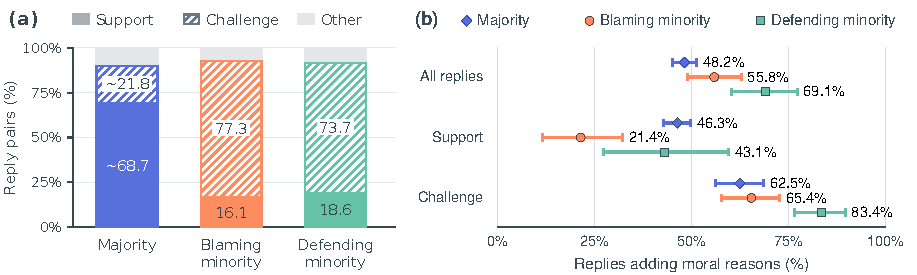
\includegraphics[width=\linewidth]{figures/aita_reply_orientation_perspectives.pdf}
  \caption{Replies to majority and blaming/defending minority comments
  in high-agreement posts. (a) Pair-weighted reply stances; Other combines
  information-seeking and other replies. (b) Post-equal percentages of
  replies with at least one moral-reason category absent from the parent,
  shown for all replies and separately for support and challenge
  (7,023 pairs; 100 posts). Whiskers: $95\%$ post-bootstrap CIs.
  Panels use separate annotation samples.}
  \label{fig:reply-responses}
  \Description{Panel a shows stacked support, challenge, and other reply
  proportions. Panel b shows means and 95 percent confidence intervals
  for addition of moral reasons in all replies, support replies, and challenge
  replies. Blue diamonds, orange circles, and green squares identify
  majority, blaming minority, and defending minority parents. Challenges
  have higher observed addition rates than support in each group.
  Defending minority parents have the highest overall and challenge-specific
  addition rates; blaming minority parents have the lowest support-specific rate.}
  \end{minipage}\hfill
  \begin{minipage}[t]{0.42\textwidth}
  \vspace{0pt}
  \centering
  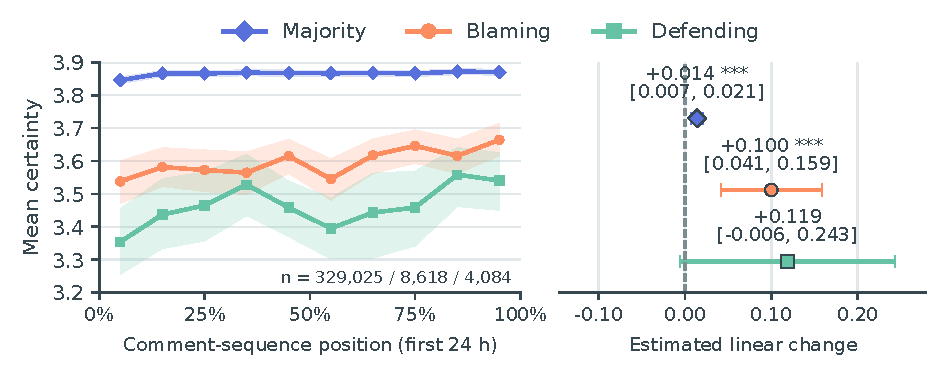
\includegraphics[width=\linewidth]{figures/fig3_certainty.pdf}
  \vspace{-14pt}
  \caption{Expressed certainty (1--4) in high-agreement posts.
  Left: post-equal means across ten stages, each containing approximately
  equal numbers of first-day comments within a post. Right: estimated
  linear change from first to last stage using all ten stages.
  Bands/whiskers: $95\%$ post-bootstrap CIs;
  stars: $^{***}p<.001$ (Holm-adjusted); $n$: comments in legend order.}
  \label{fig:aita-certainty-progress}
  \Description{Mean expressed certainty across first-day comment stages
  and estimated linear changes from post fixed-effects regression for
  majority, blaming minority, and defending minority comments.}

  \end{minipage}

\end{figure*}